Vector form of the equation of circle is :
\begin{align}
\vec{x}^T\vec{x}+2\vec{x}^T\vec{u}+f=0\label{eq:solutions/17/17/eq:1}
\end{align}
For $\vec{x_1}$, $\vec{x_2}$ and $\vec{x_3}$ equation \eqref{eq:solutions/17/17/eq:1} can be written as:
\begin{align}
\vec{x_1}^T\vec{x_1}+2\vec{x_1}^T\vec{u}+f=0\\
\vec{x_2}^T\vec{x_2}+2\vec{x_2}^T\vec{u}+f=0\\
\vec{x_3}^T\vec{x_3}+2\vec{x_3}^T\vec{u}+f=0
\end{align}
In matrix form this can be written as :
\begin{align}
    \myvec{2\vec{x_1}^T&1\\2\vec{x_2}^T&1\\2\vec{x_3}^T&1}\myvec{\vec{u}\\f}&=\myvec{-\vec{x_1}^T\vec{x_1}\\-\vec{x_1}^T\vec{x_1}\\-\vec{x_3}^T\vec{x_3}}\label{eq:solutions/17/17/eq:5}
\end{align}
By putting the values of $\vec{x_1},\vec{x_2}$ and $\vec{x_3}$ from \eqref{eq:solutions/17/17/eq:0} in \eqref{eq:solutions/17/17/eq:5} we get :   
\begin{align}
 \myvec{2&2&1\\4&-2&1\\16&4&1}\myvec{\vec{u}\\f}&=\myvec{-2\\-5\\-68} \label{eq:solutions/17/17/eq:6}
\end{align}
Using Gaussian Elimination method :
\begin{align}
\xleftrightarrow[R_2 \leftarrow R_2-4R_1]{R_1 \leftarrow \frac{1}{2}R_1}\myvec{1&1&\frac{1}{2}&-1\\0&-6&-1&-1\\16&4&1&-68}\\
\xleftrightarrow{R_3 \leftarrow R_3-16R_1}\myvec{1&1&\frac{1}{2}&-1\\0&-6&-1&-1\\0&-12&-7&-52}\\
\xleftrightarrow[R_3 \leftarrow R_3+124R_2]{R_2 \leftarrow -\frac{1}{6}R_2}\myvec{1&1&\frac{1}{2}&-1\\[0.2cm]0&1&\frac{1}{6}&\frac{1}{6}\\[0.2cm]0&0&-5&-50}\label{eq:solutions/17/17/eq:9}
\end{align}
Using \eqref{eq:solutions/17/17/eq:6} and \eqref{eq:solutions/17/17/eq:9} we get : 
\begin{align}
\myvec{\vec{u}\\f}&=\myvec{-\frac{9}{2}\\[0.1cm]-\frac{3}{2}\\[0.1cm]10}\\
\vec{u}&=\myvec{-\frac{9}{2}\\[0.1cm]-\frac{3}{2}}\\
f&=10   
\end{align}
By putting the values of $\vec{u}$ and f in \eqref{eq:solutions/17/17/eq:1} we get : 
\begin{align}
\vec{x}^T\vec{x}+2\myvec{-\frac{9}{2}\\[0.1cm]-\frac{3}{2}}^T\vec{x}+10&=0\label{eq:solutions/17/17/eq:14}\\
x^2+y^2-9x-6y+10&=0\label{eq:solutions/17/17/eq:15}
\end{align}
Plot of the circle given by equation \eqref{eq:solutions/17/17/eq:15} is as follows :
\begin{figure}[h]
\centering
    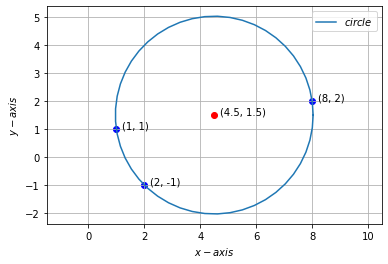
\includegraphics[width=\columnwidth]{solutions/17/17/circle3.png}
    \caption{A circle centered at $(4.5, 1.5)$ with radius $3.53$.}
    \label{eq:solutions/17/17/circle}
\end{figure}

